\section{Onion Routing and Tor}
\label{sec:tor}
Tor is an implementation of the onion routing architecture model. The
onion routing consists in a technique that provides anonymous
connections over a computer network\cite{or}.
The connections exist in three phases:
\begin{itemize}
	\item \textbf{Connection Setup}: adflkgjdflkg
	\item \textbf{Data Movement}: sfdsgdfgdf
		\begin{figure}[H]
			\centering
			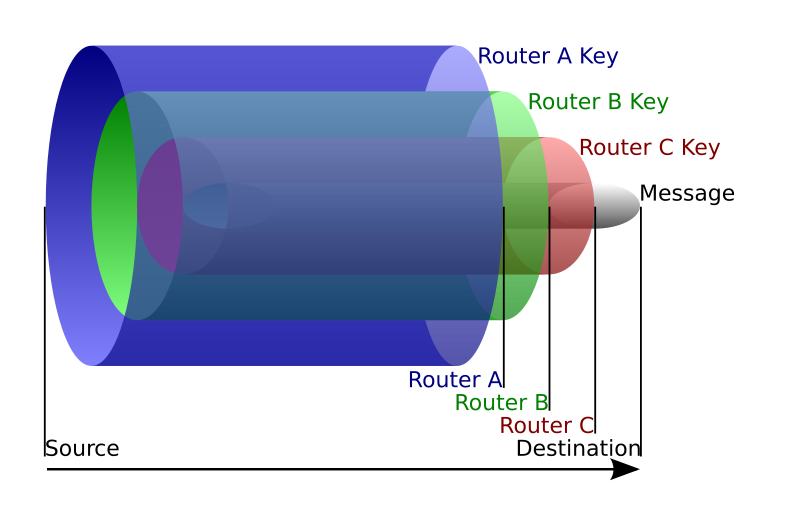
\includegraphics[scale=0.35]{onion.png}
			%TODO\caption{Add caption for this figure}
			\label{fig:onion}
		\end{figure}	
	\item \textbf{Connection Tear-Down}: sdfdjgl
\end{itemize}

\subsection{Tor architecture overview}
%TODO protects you from traffic analysis
%https://www.torproject.org/about/overview.html.en
\subsection{Tor attacks}

\subsection{Timing Attack}
